\chapter{From a Fertilized Egg to a Body}

\begin{kaichang}
The next time someone cracks a raw egg at home, do not scramble it immediately. Gently tip the yolk onto a flat plate and examine its surface. Chances are you will find a tiny white spot, only two or three millimeters across, like a grain of rice stuck to the yolk. Poultry keepers call it the ``germinal disc.''

If the egg has been fertilized and incubates at the right temperature for twenty-one days, that white spot, scarcely larger than a sesame seed, will develop into a complete chick: a beating heart, a shell-pecking beak, two eyes, and a coat of down, ready to hatch. No ``assembly'' has taken place; nobody has inserted parts. A chick simply ``grows'' from a tiny spot.

Take a guess: how do cells in that spot ``know'' which end should develop a head, where the eyes belong, or why the heart should sit a little to the left? Keep your answer in mind and revisit it at the chapter's end. The heart of the solution is something you have already met in recent chapters: how genes are switched on and off.
\end{kaichang}

\section{No ``Tiny Chick'' Inside the White Spot}

Let us begin with something people got wrong for more than two thousand years.

Before microscopes, people could see only the outcomes: eggs hatched into birds, seeds grew into trees, and pregnant women's bellies gradually enlarged. A perfectly natural guess therefore spread: perhaps that white spot, sperm, or egg already contained a miniature complete chick, and development simply ``inflated'' it. This idea is called \emph{preformationism}. In the seventeenth century, some microscopists even claimed to see curled-up ``little people'' inside sperm and solemnly drew them.

If preformationism were correct, there would be little to investigate about development: everything would already be drawn, awaiting enlargement. But as microscopes improved, observers watching rapidly changing frog eggs and chick embryos saw not miniature animals growing larger but a series of events that \textbf{created something new}: a sphere became a mass of cells; the cell ball indented and folded, forming grooves and tubes; some areas bulged and others separated. Structures were built step by step during the process and had not existed beforehand. This view, called \emph{epigenesis}, is correct. Development is not printing a photograph; it is construction on site.

Where is the construction site? Right in our opening white spot. In a fertilized chicken egg, the germinal disc is the fertilized egg and the small patch of cells produced by its divisions; the yolk is simply its packed lunch. The human story is similar: sperm and egg unite to form a fertilized egg, which divides while traveling along the fallopian tube, implants at about one week, and then follows a fairly precise timetable:

\begin{table}[htbp]
\centering
\begin{tabular}{ll}
\toprule
Time after fertilization & Major events \\
\midrule
Day 1 & One cell, about $0.1$ millimeters across \\
Week 1 & \shortstack[l]{Division into a ball of hundreds\\of cells; implantation} \\
Weeks 3--4 & \shortstack[l]{Cell ball folds into three layers;\\neural tube begins closing} \\
Weeks 5--8 & \shortstack[l]{Heart beats; head and tail distinct;\\fingers and toes ``sculpted''} \\
Week 9 onward & \shortstack[l]{Organs grow and become more refined;\\body mass rises from grams to kilograms} \\
\bottomrule
\end{tabular}
\end{table}

Notice the sequence: first comes the general layout---head, back, and limbs---and then the fine details. Seeing the whole before concentrating on particulars is the key to understanding development.

Zoom in one level further to the construction site at the particle scale. Every embryonic cell is the ``chemical city'' we met in Chapter 57: the nucleus stores the same DNA, ribosomes in the cytoplasm translate proteins, cytoskeletal protein fibers assemble and disassemble, and membrane receptors listen to the outside world. Development ultimately consists of tens of trillions of these cities following the same chemical rules, making different local decisions, and assembling a globally ordered body. The question thus becomes concrete: what information drives these local decisions---whether to divide or rest, what to become, where to move, and whether to live or die?

\section{One Cell Becomes Tens of Trillions}

Development's first operation is rather ``simple-minded'': divide, and divide again. You met mitosis in Chapter 64: chromosomes are copied and distributed between two daughter cells, passing on genetic information unchanged. So let us establish an important fact: almost every cell in your body, from brain cells to toenail cells, carries essentially the same DNA sequence. Differences lie not in the ``materials list'' but in ``which pages of the list are currently being used.'' Gene regulation from Chapter 70 and epigenetic memory from Chapter 74 are precisely what make cells different.

\begin{qiaoliang}
How many divisions does one cell need to build an adult? A newborn has about $2\times 10^{12}$ (two trillion) cells, and an adult about $3\times 10^{13}$ to $4\times 10^{13}$. Each division doubles the count. After $n$ rounds, $2^n \approx 4\times 10^{13}$. Taking logarithms gives $n \approx 13.6/0.3 \approx 45$. In other words, \textbf{forty or fifty rounds of division suffice to build an entire human body from one cell}. That is astonishingly few rounds---the trick is exponential growth: only a thousand cells at round 10, a million at round 20, a billion at round 30, and a trillion at round 40. Real divisions are not neatly synchronized, of course. Different regions undergo very different numbers of rounds: some cells, such as most neurons, stop dividing early, while others, such as intestinal epithelium and bone marrow, divide and renew throughout life. Chapter 59 discussed this tissue renewal. The value of an order-of-magnitude estimate is not precision but perspective: the ``workload'' of building a body is less unimaginable than it seems. The difficulty is not quantity but \emph{arrangement}.
\end{qiaoliang}

That is the chapter's real question: why do some of tens of trillions of genetically identical cells become neurons and others liver cells, all in the right places?

\section{Addresses: Coordinates Left by the Mother}

Imagine being blindfolded and dropped into an unfamiliar city. To find your position, you need coordinates. Embryonic cells do too, and their mother places the first set in the egg beforehand.

An egg cell looks spherical, but its interior is not uniform. Take the best-studied example, the fruit fly: while making eggs, the mother's body deposits specific messenger RNAs---the working copies of genes discussed in Chapter 68---and proteins \textbf{asymmetrically} at one end. The RNA for a protein called Bicoid is anchored at the egg's front end. After fertilization, it is translated, and the protein gradually diffuses toward the rear, producing a \textbf{concentration slope high at the front and low at the back}, like a drop of ink placed in one corner of a glass of water before mixing.

Such a molecule is called a \emph{morphogen}: its concentration itself conveys positional information. Cells at the embryo's front ``taste'' a high concentration, those in the middle an intermediate one, and those at the rear a low one. A cell need not see the whole embryo; measuring its local concentration tells it roughly which body region it occupies. This approach has a vivid name, the \emph{French flag model}: two concentration thresholds divide a gradient into blue, white, and red regions, each following different developmental instructions.

\begin{center}
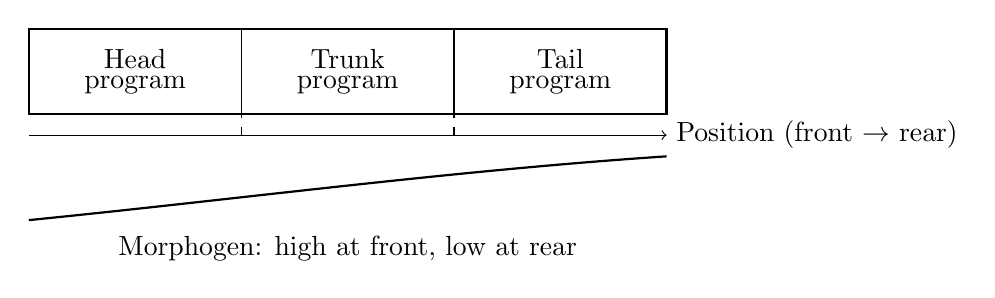
\begin{tikzpicture}[scale=0.9]
\draw[thick] (0,0) rectangle (9,1.2);
\draw (3,0) -- (3,1.2);
\draw (6,0) -- (6,1.2);
\node at (1.5,0.6) {\shortstack{Head\\program}};
\node at (4.5,0.6) {\shortstack{Trunk\\program}};
\node at (7.5,0.6) {\shortstack{Tail\\program}};
\draw[->] (0,-0.3) -- (9,-0.3) node[right]{Position (front $\rightarrow$ rear)};
\draw[thick] (0,-1.5) .. controls (3,-1.2) and (6,-0.8) .. (9,-0.6);
\node at (4.5,-1.9) {Morphogen: high at front, low at rear};
\draw[dashed] (3,-0.3) -- (3,0);
\draw[dashed] (6,-0.3) -- (6,0);
\end{tikzpicture}
\end{center}

(This is a schematic convention: real embryos have neither colors nor straight boundaries. Cells on opposite sides of a threshold statistically favor different fates.)

This ``concentration as coordinates'' logic solves a deep problem: \textbf{global patterns can arise from local rules alone}. No ``commander'' cell tells every other cell who it is. Diffusion, concentration thresholds, and cascades of gene switches allow order to grow by itself.

\section{The Gene Network's Relay Race}

Coordinates are only the beginning. Next comes an intricately choreographed relay.

In a fruit-fly embryo, maternal Bicoid protein is a transcription factor, the gene-switching character from Chapter 70. High Bicoid concentrations activate a group of ``gap genes,'' dividing the embryo into broad regions. Their products are also transcription factors, which switch the next set of genes on and off to subdivide those regions into finer stripes. Stripe genes then define segment boundaries. One layer activates the next, like spreading ripples or referees progressively dividing a racecourse. Eventually the embryo's surface is partitioned into a series of repeated segments, and every segment's cells receive their own ``segment number.''

The next relay runners are a famous group: \textbf{HOX genes}. They assign each segment an ``identity badge'': antennae here, wings there, halteres farther back. All HOX genes encode transcription factors whose protein products contain a DNA-binding structure of about 60 amino acids, called a homeodomain. They therefore resemble one another, clearly belonging to one large family.

We now need symbols for the first time in this chapter. Remember two points:

\begin{itemize}[itemsep=2pt]
\item HOX genes \textbf{form a row} on a chromosome, and their order corresponds one-to-one to their front $\rightarrow$ rear expression order in the body: the first governs the frontmost region and the last the rearmost. The chromosome's ``seating plan'' maps directly onto the body's ``floor plan.'' This is called \emph{collinearity} and remains one of developmental biology's most elegant patterns.
\item These genes are astonishingly ancient. Fruit-fly and human HOX genes are variants of the same ancestral toolkit. Humans have four clusters, \textit{HOXA}, \textit{HOXB}, \textit{HOXC}, and \textit{HOXD}, on four different chromosomes. Some human HOX genes can even partly substitute for the fly's own versions when introduced into fruit flies. Two species separated by six hundred million years of evolution still use the same ``address system'' to lay out their bodies.
\end{itemize}

HOX errors have dramatic consequences: one fruit-fly mutation gives a segment that should grow halteres---a pair of small rods that sense rotation during flight---a ``grow wings'' identity badge, producing two pairs of wings. Another mutation produces legs where antennae belong. Misplacing one gene switch puts an organ in the wrong role, demonstrating that these genes normally \textbf{specify} organ positions.

\section{Four Actions That Build a Body}

Once cells have coordinates and identity badges, what do they actually do? Development can be summarized in four basic actions:

\begin{itemize}[itemsep=2pt]
\item \textbf{Proliferation}: mitosis increases cell numbers exponentially, with forty or fifty rounds sufficient, as calculated above. Which regions divide quickly or slowly directly determines organs' relative sizes.
\item \textbf{Differentiation}: the same genome follows different operating plans. Combinations of transcription factors determine which genes a cell turns on or off, ultimately making it a neuron, muscle cell, or skin cell. Chapter 74's epigenetic modifications ``remember'' the decision, so descendants of liver cells remain liver cells.
\item \textbf{Migration}: cells ``move house.'' In vertebrate embryos, a population called the neural crest leaves the dorsal neural tube and travels throughout the body to become facial bones, pigment cells, and some nerves. Your face's shape depends partly on whether several groups of cells followed the correct routes during a few weeks of ``hiking.''
\item \textbf{Apoptosis}: programmed cell death. This is no accident; it is a \textbf{construction technique}. Human fingers are ``sculpted'' this way: the early embryonic hand is a continuous ``paddle,'' and cells between future fingers undergo coordinated apoptosis, separating the five digits. A slight malfunction in this program produces fused fingers. Many neurons also exit on schedule during brain development: overproduction comes first, followed by elimination according to connection quality.
\end{itemize}

All four actions are coordinated by gene networks and in turn change cells' positions and neighbors, altering the next round of signals. Development advances through these repeated cycles, a dynamic process that no static ``blueprint'' can contain.

The most immediate everyday evidence lies in a wound. After a scrape, cells at its edges receive signals and begin proliferating to fill the gap, migrating toward the center, and differentiating into new skin cells; surplus cells are then removed. The same four actions repeat on a much smaller scale. Development never truly ``ends''; it shifts from intensive construction to low-intensity maintenance, the lifelong renewal and homeostasis discussed in Chapters 59 and 60.

\section{Mechanics and Environment Also Shape Us}

By now you might think form is written entirely in genes. But two other hands help shape it.

The first is \textbf{mechanics}. Cells are not isolated particles floating in soup: they adhere, push, pull, and compress one another. An early embryo undergoes an astonishing transformation: a sheet of cells indents and rolls inward, like pressing in one side of a balloon, forming the primitive gut and distinguishing the body's inside from its outside. The driving forces come from cytoskeletal contraction (Chapter 57) and changes in cell adhesion---purely physical forces. Conversely, cells can ``feel'' pulling: compressed tissues alter gene expression. Bones result from this cycle; regions under frequent pressure grow thicker. Genes set the stage for mechanics, and mechanics feeds back to genes.

The second is \textbf{environment}. Temperature, nutrition, and chemicals can all intervene in development. Crocodile and sea-turtle sex is determined not by chromosomes but by incubation temperature: a difference of two or three degrees Celsius changes a clutch's sex ratio. A sobering medical lesson came in the mid-twentieth century: an anti-nausea drug called thalidomide was widely used for morning sickness and caused severe limb-development damage in more than ten thousand infants. It interfered precisely during the weeks when limbs rapidly took shape. This event directly prompted modern systems for reviewing medicines in pregnancy. It also illustrates a principle: \textbf{a developing body is extremely sensitive to disruption, with tightly defined windows of vulnerability}. The same disturbance two weeks earlier or later can have entirely different consequences. That is why doctors take medicines and nutrition during pregnancy---such as folic-acid supplementation to prevent neural-tube closure defects---so seriously: dose, timing, and individual differences can each alter the construction process.

\textbf{Translator safety note:} This teaching timeline cannot assess an individual's pregnancy exposure. Ask a doctor, midwife, or pharmacist about a specific medicine or exposure, and do not stop prescribed treatment without professional advice; stopping can also cause harm. See \href{https://www.nhs.uk/pregnancy/keeping-well/medicines/}{NHS medicines-in-pregnancy guidance}.

\begin{shiyan}
\textbf{Observation: Find an Egg's Germinal Disc} (safe to do at home)

Materials: one or two raw eggs, a flat plate, and an optional flashlight.

Procedure: (1) Gently crack the egg and slide the intact yolk onto the plate without puncturing it. (2) Look for the grayish-white circular spot, two or three millimeters across, on the yolk: the germinal disc. (3) Turn off the overhead light and illuminate the yolk from the side with a flashlight to see the disc more clearly. (4) Compare it with the two white spiral ``cords'' in the egg white, the chalazae, which anchor the yolk and are not embryos.

What to observe: how small is the germinal disc compared with the yolk? Most supermarket eggs are unfertilized, and their discs are tiny white spots. In a fertilized egg, such as one from a farm's free-range chickens, the spot is slightly larger with a more regular outline. What information must such a tiny spot use to develop a chick's complete layout?

Safety reminder: raw eggs may carry Salmonella. Wash your hands afterward, and either cook the egg thoroughly before eating it or discard it. Do not eat it raw.
\end{shiyan}

\textbf{Translator safety note:} Keep raw egg away from ready-to-eat food, wash contacted equipment and surfaces, and discard experimental samples rather than treating this observation as food preparation. See \href{https://www.fda.gov/food/retail-food-industryregulatory-assistance-training/assuring-safety-eggs-and-menu-and-deli-items-made-raw-shell-eggs}{FDA raw-egg precautions}.

\section{How Scientists Found Out: Dissecting Fly Development}

\begin{zhengju}
In the late 1970s, developmental biology faced an awkward situation: everyone had only vague guesses about how embryos formed patterns and segments. Some proposed chemical gradients, others suggested cells counted time, and everyone argued---because nobody knew which genes were involved.

In a laboratory in Heidelberg, Germany, geneticists Nüsslein-Volhard and Wieschaus chose the most ``simple-minded'' yet thorough approach: \textbf{saturation screening}. Their idea was that disabling a gene essential for development would kill the embryo at some stage, and the way it died---its pattern and segment defects---would reveal the gene's normal job. They fed male fruit flies a mutagen, which chemically damages DNA at random, as Chapter 72 explained, then crossed successive generations. Finally, they collected embryos that were \textbf{homozygous mutants and died during embryogenesis}, examining their skin patterns one by one under a microscope.

This was physically demanding work: they screened thousands of mutant lines and tens of thousands of embryos. The payoff was enormous. They identified a group of ``segment-polarity genes'': some mutant embryos had half the normal number of segments, some showed mirror-image pattern repetition within each segment, and others lacked an entire stripe. Defects corresponded clearly to normal patterns. In other words, embryonic patterns did not arise chaotically but were \textbf{controlled hierarchically} by a finite, enumerable set of genes. The ``maternal gradient---broad regions---stripes---segments'' relay described earlier was reconstructed from the death patterns of these mutants.

Alternative explanations were eliminated one by one. If the defects were merely artifacts of generalized poisoning, all mutants should have died in similar ways rather than displaying distinctive, reproducible patterns. If gradients were imaginary, later scientists disproved that suggestion by making antibodies to Bicoid and staining a real gradient, high at the front and low at the rear. Experimentally changing Bicoid levels in eggs enlarged or shrank embryonic head structures, fulfilling the prediction. This work received the 1995 Nobel Prize in Physiology or Medicine.

The story had a second act. HOX mutations that Lewis had studied for years, including four-winged flies, connected with these stripe genes: first establish segments, then assign their identities. As molecular biology matured, researchers found the same gene families in mice, humans, and even sea urchins. The ``scalpel'' applied to fruit flies had opened up a developmental toolkit shared throughout the animal kingdom. This is the chapter's central methodological lesson: \textbf{to understand a machine, one of the sharpest approaches is to break its parts one at a time and see how it fails}.
\end{zhengju}

\textbf{Translator safety note:} The mutagen-feeding study is research history, not a home or classroom procedure. Do not obtain or administer mutagens; any such work requires an appropriately equipped laboratory, trained supervision, and formal risk assessment. See \href{https://institute.acs.org/acs-center/lab-safety/education-training/safer-experiments.html}{ACS experiment-safety guidance}.

\section{Where This Explanation Has Limits}

This chapter's model is useful, but remember its boundaries.

First, \textbf{fruit flies are a special case, not the universal answer}. An early fly embryo is a ``syncytium'' sharing one cytoplasm: nuclei divide repeatedly before being partitioned into separate cells. Morphogens can diffuse freely through that common cytoplasm, making gradients especially easy to establish. Human and mouse embryos have separate cells from their first division; positional information relies more on signals passed between cells, with one releasing and its neighbor receiving. Their mechanisms resemble the fly's without being identical. Direct extrapolation from flies to humans can lead you astray.

Second, \textbf{``concentration thresholds'' are a simplification}. Real embryonic cells read not one morphogen concentration but combinations of signals, their duration, and even their rhythms of change. The French flag model captures the essence of ``position determines fate'' without encompassing every detail.

Third, \textbf{even knowing the gene network cannot predict every fingerprint}. Development includes genuine randomness: molecular fluctuations in gene expression, the stochastic differences between individual cells mentioned in Chapter 70, and tiny differences in migration paths can accumulate and amplify. Identical twins have exactly the same genes but different fingerprints and different luck with some diseases. This marks a firm boundary: DNA is not program code that completely determines a person. The chapter explains ``how a body reliably develops its general layout,'' not ``how every detail is fixed in advance.''

\begin{wuqu}
``Genes are the body's architectural blueprints; development just builds to plan.'' This widely used analogy misleads in three major ways. First, blueprints exist in full before construction, yet no embryonic location stores a ``whole-body picture.'' Cells know only local rules---measure concentrations and listen to neighbors---from which the global pattern emerges. Second, a blueprint could be torn in half to build half a building from each piece, yet in 1891 Driesch separated a two-cell sea-urchin embryo and each half developed into a complete, smaller larva. Each cell carries ``all the rules,'' not ``half a drawing.'' Third, building from blueprints is one-way execution, whereas development is a dialogue: mechanics, nutrition, and temperature feed back to modify gene-expression plans. A better analogy makes the genome a cookbook collection plus kitchen rules. The dish depends on available ingredients, the cook's (cell's) position, and the heat: the same rules yield different products in different locations.
\end{wuqu}

\section{Another Look at the Little White Spot}

Return to the opening egg. No cell in its germinal disc has ever ``seen'' a whole chicken. What the cells possess is simply asymmetric molecules deposited before the mother laid the egg; front--rear and back--belly coordinates established after fertilization; waves of diffusing signals; layer upon layer of transcription-factor relays; segment identities issued by the HOX family; and four actions---division, differentiation, moving, and programmed departure---repeated amid the pushes and pulls of mechanics and environment.

The head forms at the front because cells there read ``front'' coordinates and activate the head program. The heart sits leftward because a layer of early embryonic cells delivers a signaling molecule only to the left side; details of this ``left--right symmetry breaking'' remain debated. The eyes occupy symmetrical positions because cells on both sides read matching coordinates. No commander, no blueprint: only local rules and a relay sequence refined over hundreds of millions of years. That is how a chick grows from a white spot.

The same applies to you. You were once a cell about $0.1$ millimeters across. Forty or fifty rounds of division, countless switch changes, and several carefully arranged episodes of apoptosis produced the body now reading this book. Your navel is the commemorative medal left by that construction project.

\section{One Step Further: Where the Toolkit Came From}

Understanding development is changing medicine. Scientists can already reproduce some developmental signals in dishes using stem cells, whose pluripotency Chapter 59 discussed, to grow ``organoids'': rice-grain-sized cell clusters that partly mimic early gut, retinal, or even brain structures. They help researchers study disease and test drugs without involving actual embryos. Preventing congenital malformations, such as through folic-acid supplementation during pregnancy, and strictly managing medicines during sensitive developmental periods also rest on this chapter's picture.

But notice a huge fact left unexplained: the developmental toolkit is \textbf{astonishingly ancient}. Fruit flies and you share the same HOX toolkit. A key eye-development switch is almost interchangeable among flies, mice, and humans: activate the corresponding mouse gene in the wrong place on a fly's wing, and a fly-type eye develops there. The basic rules for building bodies have barely been rewritten over hundreds of millions of years of divergence; they have chiefly been recombined and rescheduled.

An unavoidable question remains: where did this toolkit originate? Gene sequences change as they pass down generations, through Chapter 72's mutations. Some changes alter developmental timing and location, gradually transforming one kind of animal into another. What ``selects'' these changes? How do they accumulate into the gulf between species? That is the story of Part Ten and the next chapter, Chapter 76, ``Natural Selection Is Not `Evolving Through Effort.''' Development is genes' performance within a single generation; evolution is the script's revision history over millions of generations.

\begin{tiaozhan}
Morphogen gradients explain ``high at the front, low at the rear'' coordinates, but not another common pattern: zebra stripes, leopard spots, or five fingers side by side. These \textbf{periodically repeating} structures cannot be carved out of one monotonic slope alone. In 1952, mathematician Turing---yes, the Turing of computer science---proposed an astonishing solution. Imagine two chemicals: an activator promotes both itself and an inhibitor; the inhibitor suppresses only the activator but diffuses faster. An accidental local rise in activator therefore reinforces itself into a ``peak,'' while the faster-spreading inhibitor it produces creates a surrounding ``valley.'' Peaks automatically maintain a fixed spacing, generating spots or stripes without preexisting coordinates. The mathematics of this ``reaction--diffusion'' mechanism uses just two rules: self-activation and ``inhibition spreading faster than activation.'' Fish stripes widen as fish grow, and interrupted zebrafish stripes reconnect as predicted. More than half a century later, experiments have gradually substantiated Turing's purely mathematical proposal. The details require differential equations, and skipping them will not lose the main thread. Remember the idea: \textbf{patterns need no blueprint, only the right local rules}.
\end{tiaozhan}

\section*{Try It Yourself}

\begin{sikaoti}
\item Draw an information-flow diagram beginning with ``mother places Bicoid RNA at the egg's front end'' and ending with ``cells in one embryonic region acquire segment identity.'' Include at least four stages and label each arrow as diffusion, transcription, translation, or gene switching.
\item Use the method in the text to estimate how many more division rounds an organ needs to grow from 1,000 cells to about one million. ($2^{10} \approx 10^{3}$ lets you calculate mentally.)
\item Driesch separated a two-cell sea-urchin embryo, and each half developed into a complete individual. What would the ``blueprint'' analogy predict? Why can this experiment refute preformationism without refuting the importance of genes?
\item A pregnant woman, unaware of her pregnancy, encounters the same developmental disruptor in week 4 and week 20. Using the timetable, predict which exposure carries greater risk and explain what a ``sensitive window'' means.
\item Human fingers are ``sculpted'' by apoptosis. Suggest two more examples in bodily development that might use a ``produce excess, then eliminate'' strategy: one in the nervous system and one in the immune system, revisiting Chapter 61 if helpful. Explain why this apparent waste might be reasonable.
\item Sketch HOX gene ``collinearity,'' placing chromosome gene order on the horizontal axis and front--rear body position on the vertical axis. Show how gene order corresponds to expression position and state beside the sketch that this is a representation.
\end{sikaoti}

\textbf{Translator safety note:} Exercise 4 lacks the substance, dose, and exposure details needed to rank actual pregnancy risks. It is a conceptual timing question, not a clinical assessment; later exposure is not automatically safe. Seek individualized advice and do not change prescribed treatment on the basis of this exercise. See \href{https://www.nhs.uk/pregnancy/keeping-well/medicines/}{NHS pregnancy medicine guidance}.
